

%\def \fgw {1.77in}
\def \fgw {2.7in}


\begin{figure}

\vminten

\centerline{
%\hmina
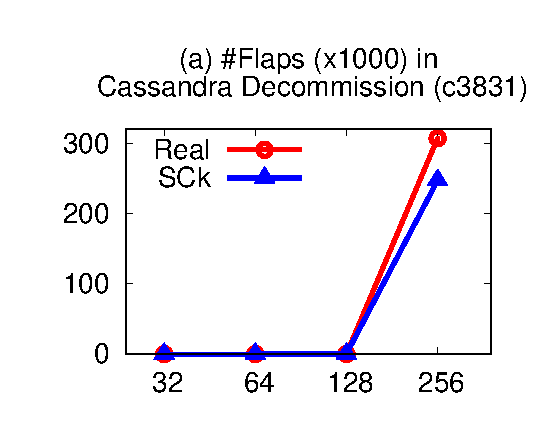
\includegraphics[width=\fgw]{F/old-bugs/eps/cass2.eps}
%\hminb
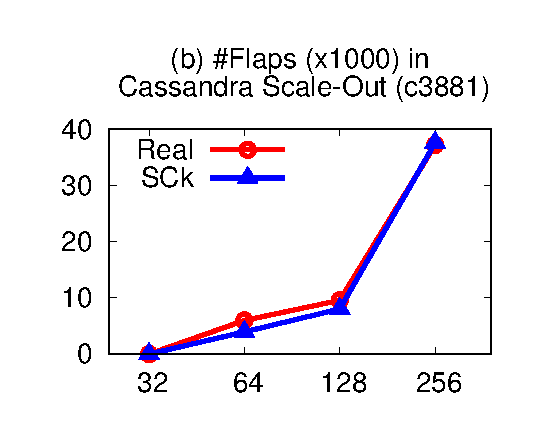
\includegraphics[width=\fgw]{F/old-bugs/eps/cass3.eps}
}

\centerline{
%\hmina
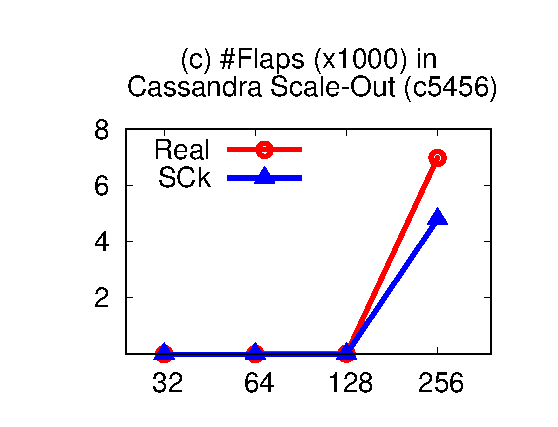
\includegraphics[width=\fgw]{F/old-bugs/eps/cass4.eps}
%\hminb
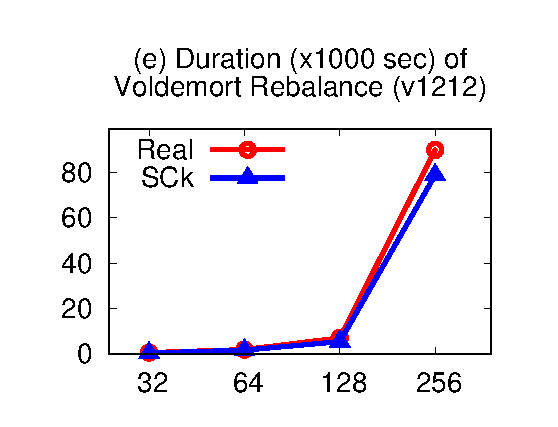
\includegraphics[width=\fgw]{F/old-bugs/eps/vold1.eps}
}

\centerline{
%\hmina
%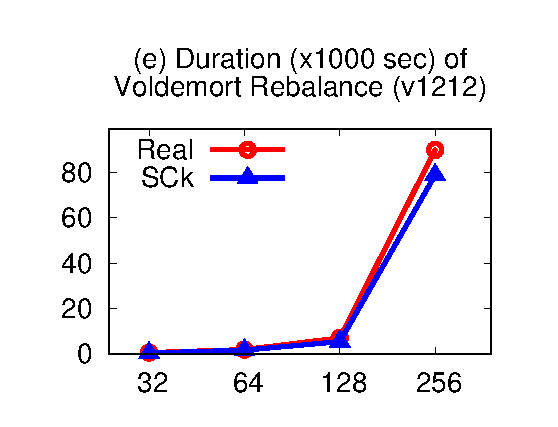
\includegraphics[width=\fgw]{F/old-bugs/eps/vold1.eps}
%\hmina
%\hminb
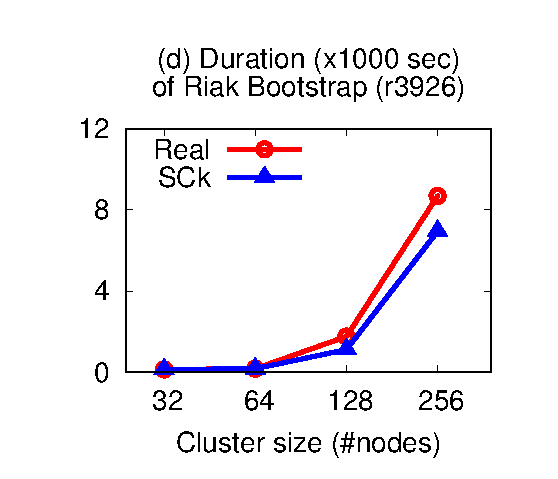
\includegraphics[width=\fgw]{F/old-bugs/eps/riak1.eps}
%\hminb
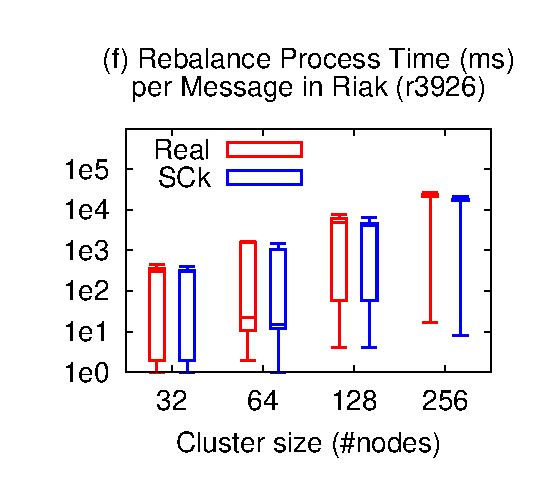
\includegraphics[width=\fgw]{F/riak/eps/proc.eps}
}

\vminfive

\mycaption[Accuracy in reproducing other bugs]({fig-bugs}{Accuracy in
reproducing other bugs}{The figures represent the bugs described in Table
\ref{tab-bugs}.  The title represents the y-axis.  We cap the y-axis to show
the scale at which the bug symptoms start to appear. }
\vminfive
\end{figure}



\if 0

TODO: CASS2: waiting for NOme to go up.
Meanwhile doing CASS3. 
%
RIAK: Buggy done, but need to plug in data from new version
(Cesar is adding fixed/patched line from the newest version).
%
VOLD: (Wait until all features are in).  Still running.
\fi
